% !TEX program = xelatex
\documentclass[10pt,a4paper]{article}

\usepackage[a4paper,left=1.45cm,right=1.45cm,top=1.15cm,bottom=1.05cm]{geometry}
\usepackage{fontspec}
\usepackage{xeCJK}
\usepackage{graphicx}
\usepackage{array}
\usepackage{tabularx}
\usepackage{enumitem}
\usepackage{xcolor}
\usepackage{titlesec}
\usepackage[hidelinks]{hyperref}
\usepackage{microtype}

% macOS 自带字体。若在其他系统编译，可替换成 Noto Sans CJK SC。
\setmainfont{Helvetica Neue}
\setsansfont{Helvetica Neue}
\setCJKmainfont{Hiragino Sans GB}
\setCJKsansfont{Hiragino Sans GB}

\definecolor{Accent}{HTML}{155E75}
\definecolor{Heading}{HTML}{17212B}
\definecolor{Muted}{HTML}{59636E}
\definecolor{Rule}{HTML}{BCD1D8}

\pagestyle{empty}
\setlength{\parindent}{0pt}
\setlength{\parskip}{0pt}
\setlength{\tabcolsep}{0pt}
\linespread{0.98}
\AtBeginDocument{\fontsize{10.1pt}{14.5pt}\selectfont}

\titleformat{\section}
  {\Large\bfseries\color{Heading}}
  {}{0pt}{}
  [\vspace{1.5pt}\color{Rule}\titlerule]
\titlespacing*{\section}{0pt}{9.5pt}{5.5pt}

\setlist[itemize]{
  leftmargin=1.35em,
  label=\textcolor{Accent}{\raisebox{0.15ex}{\scriptsize\textbullet}},
  itemsep=1.3pt,
  topsep=2.0pt,
  parsep=0pt,
  partopsep=0pt
}

% ===== 常用字段：调整简历时优先修改这里 =====
\newcommand{\ResumeName}{潘少峰}
\newcommand{\ResumePhone}{13312834541}
\newcommand{\ResumeEmail}{pan102887@gmail.com}
\newcommand{\ResumeTarget}{Java 后端开发工程师}
\newcommand{\ResumeCity}{深圳}

% 是否显示头像：改成 \showphotofalse 即可隐藏。
\newif\ifshowphoto
\showphototrue

\newcommand{\contactsep}{\hspace{0.55em}\textcolor{Rule}{|}\hspace{0.55em}}

\newcommand{\resumeheader}{%
  \ifshowphoto
    \begin{minipage}[c]{0.78\textwidth}
        {\fontsize{25pt}{28pt}\selectfont\bfseries\color{Heading}\ResumeName}\par
        \vspace{3pt}
        {\color{Muted}男 · 28 岁\contactsep 5 年工作经验\contactsep \ResumeCity}\par
        \vspace{1.5pt}
        {\color{Muted}\ResumePhone\contactsep
          \href{mailto:\ResumeEmail}{\ResumeEmail}\contactsep 求职方向：\ResumeTarget}
    \end{minipage}\hfill
    \begin{minipage}[c]{0.18\textwidth}
      \raggedleft
      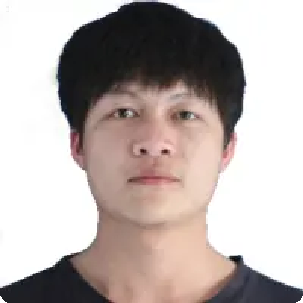
\includegraphics[width=2.22cm,height=2.22cm,keepaspectratio]{assets/photo.png}
    \end{minipage}
  \else
    {\fontsize{25pt}{28pt}\selectfont\bfseries\color{Heading}\ResumeName}\par
    \vspace{3pt}
    {\color{Muted}男 · 28 岁\contactsep 5 年工作经验\contactsep \ResumeCity}\par
    {\color{Muted}\ResumePhone\contactsep
      \href{mailto:\ResumeEmail}{\ResumeEmail}\contactsep 求职方向：\ResumeTarget}
  \fi
  \vspace{2pt}
}

% 公司/项目/学校条目标题。
\newcommand{\entry}[4]{%
  \begin{tabularx}{\textwidth}{@{}X r@{}}
    \textbf{\color{Heading}#1}\if\relax\detokenize{#2}\relax\else
      \quad {\color{Muted}#2}\fi
    & {\color{Muted}#3}\\[-1pt]
    \multicolumn{2}{@{}l@{}}{\color{Muted}#4}
  \end{tabularx}
  \vspace{1pt}
}

\begin{document}
\resumeheader
\section{个人优势}
\begin{itemize}
  \item 5 年 Java 后端研发经验，长期负责小鹏汽车商城订单、营销优惠及用户触达等核心系统建设，具备分布式微服务设计和线上系统维护经验。
  \item 具备高并发系统优化经验，基于 Kafka 完成订单链路异步化改造，将核心接口平均响应时间由 3 秒降低至 800 毫秒。
  \item 熟悉 JVM、JMM、GC 与 Java 并发编程，具备线上 CPU 高占用、OOM 等问题的定位和处理经验。
  \item 熟练使用 MySQL，具备索引设计、执行计划分析和慢查询优化经验，曾将核心查询效率提升 30\% 以上。
  \item 熟练使用 Redis 和 Kafka，具备分布式锁、限流、消息可靠投递、消费幂等及性能调优实践。
  \item 熟悉 Spring Boot、Spring Cloud 等微服务技术栈，能够独立完成技术方案设计、核心功能开发及上线保障。
\end{itemize}

\section{工作经历}
\entry{广州小鹏汽车科技有限公司}{后端开发工程师}{2021.04 -- 至今}{}
\begin{itemize}
  \item 负责小鹏汽车商城系统研发与维护，参与订单核心系统、优惠券与活动折扣、用户触达等模块建设，保障系统稳定高效运行。
  \item 分析并优化系统性能瓶颈，为重大市场活动提供技术保障，确保系统在高负载下的稳定性与响应速度。
  \item 负责小鹏汽车官网、小程序等平台的功能迭代与日常维护。
\end{itemize}

\section{项目经历}

\entry{基于 Kafka 消息队列的订单系统异步化重构}{研发工程师}{2025.01 -- 2025.02}{}
\begin{itemize}
  \item \textbf{项目背景：}订单处理系统在高并发场景下存在明显性能瓶颈，影响用户体验与业务增长；负责设计并落地订单异步处理机制，提升系统性能和可扩展性。
  \item \textbf{异步解耦：}引入 Kafka 作为消息队列，将订单流程中的非核心同步操作改造为异步处理，解耦订单服务与其他微服务之间的调用依赖，缩短核心链路并提升系统响应速度和并发处理能力。
  \item \textbf{事件驱动：}采用事件驱动架构，将订单状态变更封装为事件并通知相关服务，降低服务间耦合度，保障订单数据的一致性与处理可靠性。
  \item \textbf{项目成果：}订单处理时间减少 40\%，并发处理能力提升 60\%；部分场景下订单流程耗时缩短至原来的 1\%。
\end{itemize}

\vspace{1pt}
\entry{基于 Redis 的令牌桶限流 SDK}{研发工程师}{2024.03 -- 2024.04}{}
\begin{itemize}
  \item \textbf{项目背景：}高并发场景下的请求洪峰易造成服务不可用和用户体验下降；负责设计通用限流策略，保障系统稳定及请求的公平性与可用性。
  \item \textbf{限流实现：}采用令牌桶算法控制订单请求速率，并使用 Redis 存储共享限流状态，实现分布式限流及限流数据的高可用与一致性。
  \item \textbf{熔断保护：}系统过载时快速失败，阻断过量请求持续冲击下游服务，避免系统过载和故障扩散。
  \item \textbf{项目成果：}请求成功率提升 30\%，用户投诉减少 50\%；核心业务系统未再因流量洪峰出现服务重启或宕机，服务可用性得到提升。
\end{itemize}

\section{教育经历}
\entry{华北电力大学（保定）}{本科 · 网络工程}{2016 -- 2020}{美国大学生数学建模竞赛 M 奖}

\end{document}
